\chapter*{Kurzfassung der Diplomarbeit/Abstract} \addcontentsline{toc}{chapter}{Kurzfassung der Diplomarbeit/Abstract}

Hier bitte die ausgefüllten Formulare der Antragstellung in deutscher und englischer Sprache einfügen.

Seitennummerierung mit B,C,...

\clearpage

\newlength{\htllogobreite}
\htllogobreite29mm
\newlength{\beschriftungsbreite}
\beschriftungsbreite127mm
\newlength{\feldA}
\feldA50mm
\newlength{\feldB}
\feldB77mm

\begin{tabular}{|p{\htllogobreite}|p{\beschriftungsbreite}|}
\hline
\multirow{2}{\htllogobreite}{\epsfig{figure=images/htl_logo_beschnitten.eps, width=29mm, angle=0}}&{\vspace{0.05em}\textbf{HÖHERE TECHNISCHE LEHRANSTALT YBBS AN DER DONAU}}\\[1.05em]
\cline{2-2}
 & { \begin{tabular}{p{\feldA} p{\feldB}}
    Fachrichtung:&\textbf{Informationstechnologie}\\
    Ausbildungsschwerpunkte:&\textbf{Netzwerk- und Medientechnik}\\
   \end{tabular}
   }\\
\hline
\end{tabular}

\begin{center}
 \LARGE \textbf{DIPLOMARBEIT}\\
 \Large \textbf{DOKUMENTATION}\\
 \normalsize
\end{center}

\newlength{\feldC}
\feldC49mm
\newlength{\feldD}
\feldD107mm

\linespread{1.1} \normalsize
\begin{tabular}{|p{\feldC}|p{\feldD}|}
 \hline
 Namen der Verfasser/innen & David Pöchacker, Marcel Entner, Tobias Kronsteiner \\
 \hline
 Jahrgang Schuljahr & 5AHITN  2021/22 \\
 \hline
 Thema der Diplomarbeit &Echtzeit Visualisierung von Energiesystemen \\
 \hline
 Kooperationspartner & Bioenergy and Sustainable Technologies GmbH\\
 \hline
\end{tabular}

\begin{tabular}{|p{\feldC}|p{\feldD}|}
 \hline
 Aufgabenstellung & Das Ziel der Diplomarbeit „Echtzeit Visualisierung von Energiesystemen" ist, dem Unternehmen Best GmbH eine zentrale Verwaltung von Energiesystemen bereitzustellen. Zusätzlich zur Verwaltung soll es möglich sein, Echtzeitdaten von einer ausgewählten Energietechnologie in Form von Statistiken zu visualisieren.\\
 \hline
\end{tabular}

\begin{tabular}{|p{\feldC}|p{\feldD}|}
 \hline
 Realisierung & Die Weboberfläche wurde mit Laravel umgesetzt. Eingegebene Daten werden in einer Datenbank erfasst und mittels Grafana auf der Weboberfläche visualisiert. Abrufbar ist das Produkt über eine vom Auftraggeber bereitgestellte Domain mit dazugehörigen Webserver.  \\
 \hline
\end{tabular}

\begin{tabular}{|p{\feldC}|p{\feldD}|}
 \hline
 Ergebnisse &  Mithilfe des Produktes können Energiesysteme sowie Energietechnologien erstellt, bearbeitet und gelöscht werden. Ein rollenbasiertes Benutzersystem regelt den Zugriff auf die Verwaltung der einzelnen Energiesystemen. Der Administrator Benutzer hat als einziger die Möglichkeit neue Benutzer hinzuzufügen oder bestehende zu löschen. Jedem Benutzer ist es möglich, die Grafana Statistiken seiner selbst erstellen Energietechnologien anzeigen zu lassen.\\
 \hline
\end{tabular}

\begin{tabular}{|p{\feldC}|p{\feldD}|}
 \hline
 Architektur &  
 \rule{0pt}{3cm+1ex} 
 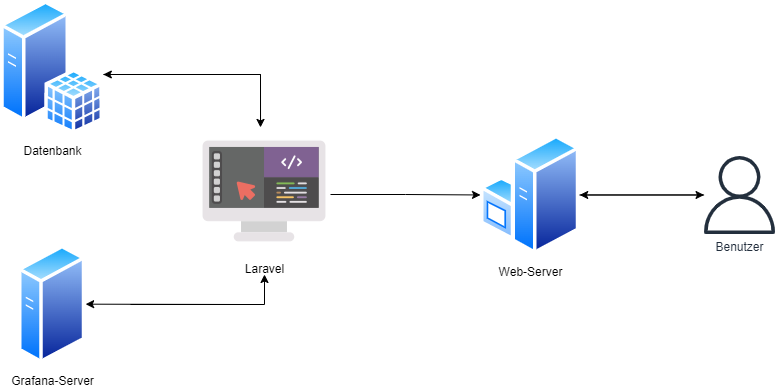
\includegraphics[height=3cm]{images/1} \\
 
 \hline
\end{tabular}


\begin{tabular}{|p{\feldC}|p{\feldD}|}
 \hline
 Teilnahme an Wettbewerben, & Mostviertler Schulinovationspreis \\
 Auszeichnungen & noch keine\\
 \hline
\end{tabular}

\begin{tabular}{|p{\feldC}|p{\feldD}|}
 \hline
 Möglichkeiten der Einsicht- & Bibliothek SZ-Ybbs \\
 nahme in die Arbeit & \\
 \hline
\end{tabular}

\newlength{\feldE}
\feldE51mm


\begin{tabular}{|p{\feldC}|p{\feldE}|p{\feldE}|}
 \hline
 Approbation \small{Prüfer}& \scriptsize{Prüfer/Prüferin} & \scriptsize{Direktor bzw. Abteilungsvorstand}\\ 
 (Datum / Unterschrift)& & \\
 \hline
\end{tabular}
\linespread{1.25} \normalsize

\clearpage

% Makro um in vorgegebener Spaltenbreite zentrieren zu können
\newcolumntype{C}[1]{>{\centering\arraybackslash}m{#1}}

\begin{tabular}{|p{\htllogobreite}|C{\beschriftungsbreite}|}
\hline
\multirow{2} {\htllogobreite} {\epsfig{figure=images/htl_logo_beschnitten.eps, width=29mm, angle=0}} & \vspace{0.05em}\textbf{HÖHERE TECHNISCHE LEHRANSTALT YBBS AN DER DONAU}\\
& \textbf{COLLEGE of ENGINEERING}\\[0.05em]
\cline{2-2}
 & { \begin{tabular}{p{\feldA} p{\feldB}}
    Department:&\textbf{Information Technology}\\
    Educational focus:&\textbf{Network and Media Technology}\\
   \end{tabular}
   }\\
\hline
\end{tabular}

\begin{center}
 \LARGE \textbf{DIPLOMA THESIS}\\
 \Large \textbf{Documentation}\\
 \normalsize
\end{center}

\linespread{1.1} \normalsize
\begin{tabular}{|p{\feldC}|p{\feldD}|}
 \hline
 Author(s) & \\
 \hline
 Form & \\ Academic year & \\
 \hline
 Topic & \\
 \hline
 Co-operation Partners & \\
 \hline
\end{tabular}

\begin{tabular}{|p{\feldC}|p{\feldD}|}
 \hline
 Assignment of Tasks & \\
 \hline
\end{tabular}

\begin{tabular}{|p{\feldC}|p{\feldD}|}
 \hline
 Realisation & \\
 \hline
\end{tabular}

\begin{tabular}{|p{\feldC}|p{\feldD}|}
 \hline
 Results & \\
 \hline
\end{tabular}

\begin{tabular}{|p{\feldC}|p{\feldD}|}
 \hline
 Illustrative Graph, Photo & \\
 (incl. explanation) & \\
 \hline
\end{tabular}

\begin{tabular}{|p{\feldC}|p{\feldD}|}
 \hline
 Participation in Competitons & \\
 Awards & \\
 \hline
\end{tabular}

\begin{tabular}{|p{\feldC}|p{\feldD}|}
 \hline
 Accessibility of Diploma Thesis & \\
 \hline
\end{tabular}

\begin{tabular}{|p{\feldC}|p{\feldE}|p{\feldE}|}
 \hline
 Approval & \scriptsize{Examiner} & \scriptsize{Head of College / Department}\\ 
 (Date / Sign)& & \\
 \hline
\end{tabular}
\linespread{1.25} \normalsize
